% ****** Start of file apssamp.tex ******
%
%   This file is part of the APS files in the REVTeX 4 distribution.
%   Version 4.0 of REVTeX, August 2001
%
%   Copyright (c) 2001 The American Physical Society.
%
%   See the REVTeX 4 README file for restrictions and more information.
%
% TeX'ing this file requires that you have AMS-LaTeX 2.0 installed
% as well as the rest of the prerequisites for REVTeX 4.0
%
% See the REVTeX 4 README file
% It also requires running BibTeX. The commands are as follows:
%
%  1)  latex apssamp.tex
%  2)  bibtex apssamp
%  3)  latex apssamp.tex
%  4)  latex apssamp.tex
%
%\documentclass[twocolumn,showpacs,preprintnumbers,amsmath,amssymb]{revtex4}
\documentclass[preprint,showpacs,preprintnumbers,amsmath,amssymb]{revtex4}


% Some other (several out of many) possibilities
%\documentclass[preprint,aps]{revtex4}
%\documentclass[preprint,aps,draft]{revtex4}
%\documentclass[prb]{revtex4}% Physical Review B

%Denton
\providecommand{\e}[1]{\ensuremath{\times 10^{#1}}}
\newcommand{\ee} {\,\text{e}}
\newcommand{\beq}{\begin{equation}}
\newcommand{\eeq}{\end{equation}}
\newcommand{\beqs}{\begin{equation*}}
\newcommand{\eeqs}{\end{equation*}}
\newcommand{\barr}{\begin{array}}
\newcommand{\earr}{\end{array}}
\newcommand{\bce}{\begin{center}}
\newcommand{\ece}{\end{center}}
\newcommand{\asymplim}[1]{\: {\underset{\scriptstyle{{#1}\to\infty}}{\displaystyle{\sim}}} \:}
\newcommand{\kr} {\kappa\rho}
\newcommand{\krp} {\kappa\rhop}
\newcommand{\mr} {\mu\rho}
\newcommand{\mrp} {\mu\rho'}
\newcommand{\rhop} {\rho'}
\newcommand{\ii}{{\rm{i}}}
%Denton
\usepackage{graphicx}% Include figure files
%\usepackage[draft]{graphicx} % Do not include figure files
\usepackage{dcolumn} % Align table columns on decimal point
\usepackage{bm} % bold math
%\usepackage{booktabs, tabularx}%toprule/bottomrule
\usepackage{todonotes}
\usepackage[hidelinks]{hyperref}  % For clickable references
%%%%%% My definitions
\def \bea{\begin{eqnarray}}
\def \eea{\end{eqnarray}}
\newcommand{\todoi}{\todo[inline]}
%%%%%% End my definitions

% Subfolders containing our images
\graphicspath{{IPython/}{Images/}}




%\nofiles
\begin{document}

\preprint{APS/123-QED}

\title {A Detailed Investigation of Low-Energy Positronium-Hydrogen Scattering}

\author{Denton Woods }
\author{S. J. Ward}
\affiliation{Department of Physics, University of North Texas}
 %\email{Second.Author@institution.edu}

\author{ P. Van Reeth}
\affiliation{Department of Physics and Astronomy, University College London, ..}
%Second institution and/or address\\
%This line break forced% with \\ }%

\date{\today}% It is always \today, today,
             %  but any date may be explicitly specified

\begin{abstract}



   \end{abstract}
   
%\pacs{Valid PACS appear here}
%\keywords{Suggested keywords}
\maketitle

\section{\label{sec:Intro}\protect Introduction}



\preprint{APS/123-QED}

\title{Detailed Investigations of Positronium-Hydrogen Collisions}

\author{Denton Woods }
\affiliation{Department of Physics, University of North Texas, Denton TX 76103-1427}
\author{and \\ S. J. Ward}%
 %\email{Second.Author@institution.edu}

%\author{Charlie Author}
% \homepage{http://www.Second.institution.edu/~Charlie.Author}
\affiliation{Department of Physics, University of North Texas, Denton TX 76103-1427}
%Second institution and/or address\\
%This line break forced% with \\ }%

\date{\today}% It is always \today, today,
             %  but any date may be explicitly specified


\noindent
NEEDS REVISIONS!!
REFERENCES ARE NOT NUMBERED CORRECTLY!
\section{Introduction}


Positronium (Ps) scattering from atoms and molecules is an area of current experimental and theoretical interest. The development of energy-tunable ortho-Ps beams [1-5] has enabled measurements
to be made of Ps scattering from the inert gases, He, Ne, Ar and Xe [5-8] and the following molecules ----. The cross sections for Ps scattering from H has not been measured due to the difficulty
of an atomic hydrogen beam, although the binding energy of positronium hydride, PsH, has been measured in the reaction of a positron with methane, e$^+$ + CH$_4$ $\to$ CH$_3^+$ + PsH [9].
However, both the UCL [10] and St.~Olaf [11] positron experimental groups have independently proposed to measure  Ps scattering from the effective one-electron atoms, the alkali atoms.
The St.~Olaf positron experimental group  plans to perform the measurements of positron-alkali atom collisions at very low energies. The low-energy region is of particular interest
because in this energy range positron and electron correlations are dominant. The proposed measurements of Ps-alkali atom at low energies initiated our recent project to investigate Ps collisions from
H and the alkali atoms using the Kohn variational method which is an appropriate method for low energy scattering. Currently, we have considered H only and it is our work of the application of the Kohn variational method
(and variants of the method) to elastic S-wave Ps-H scattering in the energies up to the excitation threshold of Ps(n=2) (5.1 eV) that we are presenting in this paper.


Ps-H scattering is a fundamental four-body Coulomb process
and is of interest in the study of solar processes [59].
As well as the basic interest of Ps-atom scattering in atomic physics,
Ps is also important in material science.
As Ps is a neutral atom, it penetrates deeper into material than a charged particle,
such as a positron.
Ps scattering also has applications
in other areas of physics such as in biophysics and astrophysics \cite{}.

The Kohn (and Inverse) variational method has previously been applied to
to Ps-H collisions by 
Van Reeth and Humberston [13,14] who computed singlet and triplet elastic
S- and P-wave elastic phase shifts. 
We have extended their S-wave Kohn variational calculation in two important ways.
First, and foremost, in addition to implementing
the Kohn and inverse Kohn variational methods, we have
implemented the generalized Kohn and the complex Kohn
for the S and T-matrices. The generalized Kohn---
The complex Kohn variational method is known to suffer
from far few anomalous singularities than the
Kohn or inverse Kohn variational method [15,Cooper ]. 
(See Cooper's papers.) (Verified the test of Cooper---T-matrix
phase shift/Kohn goes through it.)
The second extension that we considered was to use
the procedure by Todd to systematically remove terms that
were causing linear dependence.
This enabled us to compute the phase shifts (and the binding
energy of PsH) with a larger value of omega (see the method section)
and thus more short-range Hylleraas terms than the earlier 
Kohn calculation. 
This investment of time to find a procedure to find
a procedure that provides accurate results
and reduces problems with linear dependence
will be of beneficial for the higher partial waves.

Using the various of the Kohn variational method we 
computed singlet and triplet S-wave 
phase shifts and scattering lengths for Ps-H scattering.
We determined these quantities for a number of values
of omega which enabled us to
extrapolate the results to infinite omega.
This enabled us to obtain an accuracy of our results.
In addition, we confirm the two previous observed res
for the singlet S-wave, and compare the
position of the widths with the earlier Kohn calculations,
a stabilization and close-coupling calculations.
We also used the short-range part/correlation part of
the full scattering wave function to compute
the binding energy of PsH.
By comparing our result with the most elaborate
variational results gives an indication of the
reliability  of describing the Ps-H system
at short-distances.

There have been a number of other calculations for
Ps-H scattering. A much earlier Kohn variational calculation was performed
by Page [71] for the Ps-H scattering lengths.
At low energies, Diffusion Monte Carlo (DMC) [63],
the Stochastic  Variational Method (SVM) [64-66],  Close-Coupling (CC) [67-70], 
 methods have been applied.
The SVM with stabilization techniques was used to compute
accurate low-energy phase shifts and scattering lengths for Ps-H collisions [64-66].
A disadvantage of the SVM over scattering theory methods
such as the Kohn variational method is that the phase shifts
are  determined at energies which  are not  known in advance [66].
Thus,  the S- and P-wave
effective-range parameters had first to be used to compute the phase shifts at the same energy
points before the cross section could be computed [66]. 
A disadvantage of both the SVM 
and DMC  methods is that they do not  give
bounds on the scattering parameters [72].
This means that it is difficult to assess whether the results
obtained from these methods are converged with respect
to improvements in the wave function.

Blackwood et al. [69]  performed an elaborate CC calculation for Ps scattering from H which took into account excitation and ionization of both the projectile and target. They considered two different coupling schemes.
The first one, which they refer to as 9Ps9H, included 9 eigen- and pseudo-states of Ps and also of H. The second scheme, which they refer to as 14Ps14H, is for the S-wave only
and includes 14 eigen- and pseudo-states of Ps and
also of H.
Good agreement is obtained between the CC [69] and the SVM [65]
for the S-wave scattering lengths and phase shifts. Walters et al. [70]  extended the earlier CC calculations
 [69] to include the e$^+$-H$^-$ channel
and compared their results for the S-wave with the accurate
Kohn variational results [72].
They speculated that the inclusion of the virtual Ps$^-$ formation channel may
be needed to obtain agreement with the Kohn variational results
for Ps(1s) + H(1s) scattering [70].

Unlike the SVM and 
DMC methods, the Kohn
variational method gives rigorous bounds on the scattering
lengths and  except for Schwartz singularities gives empirical bounds on
the elastic phase shifts.
This means that the wave function can be systematically
improved to the converged results.
The Kohn variational method is known to yield accurate results and 
has provided benchmark results [70,72] to which results from
other calculations can be compared.
As discussed by Dr. James Walters in his  invited talk
at Posmol 2009,
the Kohn variational method has provided
valuable benchmark calculations to hang theoretical
calculations that are now coming into place.
Unlike the SVM, the method can 
treat inelastic as well as elastic scattering
and thus can be extended to higher energies. 


Goal is to provide accurate and benchmark calculations.
\vskip 0.5truecm
\noindent
\section{Theory}

\subsection{The Positronium-Hydrogen System}

%begin{figure}[!h]
%	\centering
%	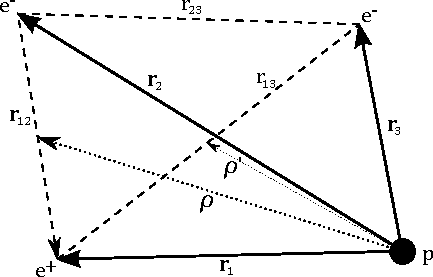
\includegraphics[height=3in]{PsHCoordinates}
%	\caption{Positronium Hydride Coordinate System}
%	\label{fig:PsHCoords}
%\end{figure}

\begin{figure}[!h]
	\centering
	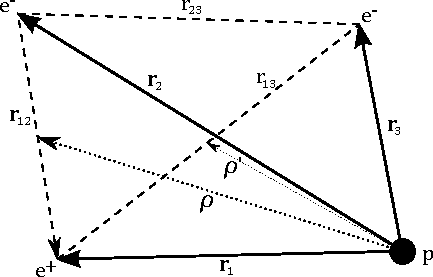
\includegraphics[height=2in]{PsHCoordinates}
	\caption{Positronium-Hydrogen Coordinate System}
	\label{fig:PsHCoords}
\end{figure}

\todoi{Do we want to state at some point that the t is implicit? Earlier versions did.}
We are investigating low-energy elastic positronium-hydrogen (Ps-H) for energies up to the excitation threshold of Ps(n=2) at approximately 5.101 eV. Previous work on Ps-H scattering used the Kohn and inverse Kohn approach \cite{VanReeth2003, VanReeth2004}. However, both of these methods are known to be sometimes affected by Schwartz singularities. In addition to using a generalized real Kohn method, to reduce the presence of Schwartz singularities, we also calculate the phase shifts using a T-matrix complex Kohn method. Both of these methods are described in sections \ref{sec:ComplexKohn} and \ref{sec:GenKohn}. All of our final results presented in section \ref{sec:Results} use the T-matrix complex Kohn method, so we present our complex-valued wavefunctions here.

For S-wave scattering of positronium from hydrogen, our very flexible \todo{Needed?} complex-valued trial scattering wavefunction is
\todoi{Need $\ell$'s? It's only one partial wave.}
\begin{equation}
\Psi^{\pm,t} = \bar{S} + T^{\pm,t} \, \bar{W} + \sum_{i=1}^N c_i \bar{\phi}_{i1},
\label{eq:TrialWave}
\end{equation}
where the superscript $t$ indicates that this is a trial wavefunction, and the $\pm$ indicates the spatially symmetric singlet and antisymmetric triplet cases. Earlier work by Van Reeth and Humberston used a real-valued trial wavefunction with the Kohn and inverse Kohn variational methods \cite{VanReeth2003, VanReeth2004}. For higher partial waves \todo{$\ell?$} $(L > 0)$,
\begin{equation}
\Psi_\ell^{\pm,t} = \bar{S_\ell} + T^{\pm,t}_\ell \, \bar{W}_\ell + \sum_{i=1}^N c_{i,\ell} \bar{\phi}_{i1} + \sum_{j=1}^N d_{j,\ell} \bar{\phi}_{j2}.
\label{eq:TrialWaveHigher}
\end{equation}
The scattering wavefunctions contain both the long-range asymptotic form and short-range correlation terms for small interparticle distances. The coordinate system used in these is shown in figure \ref{fig:PsHCoords}. The variable $\rho$ describes the position of the center of mass of the positronium atom, i.e. $\vec{\rho} = \frac{1}{2}\left(\vec{r_1} + \vec{r_2}\right)$. The long-range asymptotic terms are
\todo{1S,1s?}
\begin{subequations}
\label{eq:SCPhiDef}
\begin{align}
\bar{S}_\ell &= \frac{1\pm P_{23}}{\sqrt{2}}Y_{\ell 0}(\theta_\rho,\phi_\rho)\Phi_{Ps,1S}\left(r_{12}\right) \Phi_{H,1S}\left(r_3\right) \sqrt{2\kappa} \,j_\ell\left(\kappa\rho\right) \label{eq:SBar} \\
\bar{C}_\ell &= \frac{1\pm P_{23}}{\sqrt{2}}Y_{\ell 0}(\theta_\rho,\phi_\rho)\Phi_{Ps,1S}\left(r_{12}\right) \Phi_{H,1S}\left(r_3\right) \sqrt{2\kappa} \,n_\ell\left(\kappa\rho\right) f_\ell(\rho) \text{ and}\label{eq:CBar} \\
\bar{W}_\ell &= \bar{C}_\ell + \ii \bar{S}_\ell.
\end{align}
\end{subequations}
Note that this is different than Cooper et al.\ \cite{Cooper2010}, in that we do not use a variable $\tau$, and our $\bar{W}$ is their $\bar{T}$ but with $\bar{C}$ and $\bar{S}$ swapped, which gives an outgoing wave. $P_{23}$ is the exchange operator for the two electrons. $\Phi_{Ps,1S}\left(r_{12}\right)$ and $\Phi_{H,1S}\left(r_3\right)$ are the ground state wavefunctions of positronium and hydrogen, respectively. The shielding factor, $f_\ell(\rho)$, ensures that the singularity of the Neumann function is removed at the origin and is chosen to be
\begin{equation}
f_\ell(\rho) = \left[1 - \ee^{-\mu \rho} \left(1+\frac{\mu}{2}\rho\right)\right]^{m_\ell}.
\label{eq:PartialWaveShielding}
\end{equation}
The $m_\ell$ is an integer chosen for each $\ell$ so that $\bar{C}$ behaves like $\bar{S}$ as $\rho \rightarrow \infty$.
\todoi{behaves asymptotically as $\bar{S}$}

The short-range terms are highly correlated Hylleraas-type functions\todo{basis sets?}, given by
\begin{subequations}
\label{eq:PhiDef}
\begin{align}
\bar{\phi}_{i1} &= \left(1 \pm P_{23}\right) Y_{\ell 0}(\theta_1,\phi_1) r_1^{k_i + \ell} r_2^{l_i} r_{12}^{m_i} r_3^{n_i} r_{13}^{p_i} r_{23}^{q_i} \text{ and} \label{eq:PartialWavePhi1i}\\
\bar{\phi}_{j2} &= \left(1 \pm P_{23}\right) Y_{\ell 0}(\theta_2,\phi_2) r_1^{k_i} r_2^{l_i + \ell} r_{12}^{m_i} r_3^{n_i} r_{13}^{p_i} r_{23}^{q_i} \label{eq:PartialWavePhi2j}.
\end{align}
\end{subequations}
The variable $\omega$ is an integer $\geq 0$ that determines the maximum number of terms in the basis set. For a chosen value of $\omega$, the integer powers of $r_i$ and $r_{ij}$ are constructed in such a way that $k_i + l_i + m_i + n_i + p_i + q_i \leq \omega$, with all $k_i$, $l_i$, $m_i$, $n_i$, $q_i$ and $p_i$ $\geq 0$.

These short-range terms represent the angular momentum as being placed on either the positron ($r_1$) or on the electron on the Ps atom ($r_2$). \todoi{Mention other formalism we tried.} For partial waves with $L>1$, the angular momentum could be shared between both particles in the Ps atom \cite{??} (Schwartz). An investigation of the contribution to the final results from each symmetry for \todo{What system?} \todoi{find paper Pos-He 1999 or thesis} has revealed that the mixed symmetries were not important, and because of the complexity of the analytical evaluation of the various matrix elements, we have omitted the mixed symmetry term.


%THE HAMILTONIAN
The Hamiltonian for the fundamental Coulombic system is
\begin{align}
H = -\frac{1}{2} \nabla_{r_1}^2 - \frac{1}{2} \nabla_{r_2}^2 - \frac{1}{2} \nabla_{r_3}^2 + \frac {1}{r_1}-\frac {1}{r_2}-\frac {1}{r_3}-\frac {1}{r_{12}}-\frac {1}{r_{13}}+\frac {1}{r_{23}}
	\label{Hamiltonian1}
\end{align}
which can also be expressed in terms of the variables associated with the Ps coordinates as
\begin{align}
H = -\frac{1}{4} \nabla_{\rho}^2 - \frac{1}{2} \nabla_{r_3}^2 - \nabla_{r_{12}}^2 + \frac {1}{r_1}-\frac {1}{r_2}-\frac {1}{r_3}-\frac {1}{r_{12}}-\frac {1}{r_{13}}+\frac {1}{r_{23}}
	\label{Hamiltonian2}
\end{align}




\subsection{Complex Kohn Variational Principle (T-Matrix)}
\label{sec:ComplexKohn}

 We give the derivation of the complex Kohn variational functional for all partial waves using a complex wavefunction.

The functional for the full wavefunctions in equations \ref{eq:TrialWave} and \ref{eq:TrialWaveHigher} is
\begin{equation}
I_l[\Psi^t] = \left(\Psi^t, L \Psi^t \right) = \int \Psi^t L \Psi^t \,d\tau,
\label{eq:IlDefPsi}
\end{equation}
with
\beq
L = 2(H - E).
\label{eq:LDef}
\eeq

\todoi{We need to check about conjugation notation.}

We assume our trial wavefunction is a small variation of the exact wavefunction, or
\beq
\Psi^t = \Psi + \delta \Psi
\label{eq:PsiTrialRelation}
\eeq
Then the variation of $I_l$ to first order in $\delta\Psi_l$ is
\begin{equation}
\nonumber \delta I_l = I_l[\Psi^t] - I[\Psi] \\
\label{eq:IlPsiVariation1}
\end{equation}

It can be shown that solving for $\delta I$ gives a result for the variational method of
\beq
\delta I = (T^t - T)
\eeq
or
\beq
I[\Psi^t] - I[\Psi] = I[\Psi^t] = T^t - T.
\eeq
Neglecting the second order term, we get a functional for the variational T-matrix of
\beq
T^v = T^t - I[\Psi^t].
\label{eq:ComplexKohnVariation}
\eeq

We can use this now in the stationary property of the complex Kohn functional, i.e.
\beq
\frac{\partial T^v}{\partial T^t} = 0  \text{ and } \frac{\partial T^v}{\partial c_i} = 0 \text{ where $i = 1,\ldots,N$}.
\label{eq:ComplexKohnStationary}
\eeq
Using equations \ref{eq:TrialComplex} and \ref{eq:ComplexKohnVariation}, the stationary property in equation \ref{eq:ComplexKohnStationary} can be written in matrix form for the S-wave as
\begin{equation}
\label{eq:ComplexKohnMatrix}
\begin{bmatrix} 
 (\bar{W},L\bar{W}) & (\bar{W},L\bar{\phi}_1) & \cdots & (\bar{W},L\bar{\phi}_j) & \cdots\\
 (\bar{\phi}_1,L\bar{W}) & (\bar{\phi}_1,L\bar{\phi}_1) & \cdots & (\bar{\phi}_1,L\bar{\phi}_j) & \cdots\\
 \vdots & \vdots & \ddots & \vdots \\
 (\bar{\phi}_i,L\bar{W}) & (\bar{\phi}_i,L\bar{\phi}_1) & \cdots & (\bar{\phi}_i,L\bar{\phi}_j) & \cdots\\
 \vdots & \vdots & & \vdots & \\
\end{bmatrix}
\begin{bmatrix}
T^t\\
c_1\\
\vdots\\
c_i\\
\vdots
\end{bmatrix}
= -
\begin{bmatrix}
(\bar{W},L\bar{S}) \\
(\bar{\phi}_1,L\bar{S}) \\
\vdots \\
(\bar{\phi}_i,L\bar{S}) \\
\vdots
\end{bmatrix}.
\end{equation}

\noindent For higher partial waves, the matrix equation looks the same but includes the second symmetry short-range terms. This matrix equation can be rewritten as $\textbf{\emph{AX = -B}}$. Finally, we solve for $T^v$, from which we obtain our phase shifts.
\begin{equation}
T^v = -\textbf{\emph{B}}^{tr} \textbf{\emph{X}} - (\bar{S},L \bar{S})
\end{equation}

The T-matrix is related to the phase shift, $\delta_\ell$, and the K-matrix by
\todo{ref? K?}
\begin{equation}
\tan \delta = K^v = \frac{T}{1 + \ii T}.
\end{equation}
\todoi{Do we really need to put the superscripts here now? This applies equally to the trial and variational values.}


\subsection{Generalized Kohn Variational Method}
\label{sec:GenKohn}

We use the complex Kohn method for all of our results due to its stability, but as described in section \ref{sec:Truncation}, we also use the real-valued generalized Kohn variational method \todo{ref?} to determine how many terms we can use. The wavefunction given in (\ref{eq:TrialWaveHigherGen}) has an adjustable parameter $\tau$, which we vary. Special cases of this are the Kohn method for $\tau = 0$ and the inverse Kohn method for $\tau = \pi/2$.

\todoi{$c_i$ and $d_j$ are different from before...}
\begin{equation}
\tilde{\Psi}_\ell^{\pm,t} = \tilde{S_\ell} + \tan(\delta^{\pm,t}_\ell - \tau) \, \tilde{C}_\ell + \sum_{i=1}^N c_{i,\ell} \bar{\phi}_{i1} + \sum_{j=1}^N d_{j,\ell} \bar{\phi}_{j2}.
\label{eq:TrialWaveHigherGen}
\end{equation}
where
\begin{equation}
\begin{bmatrix}
\tilde{S} \\
\tilde{C}
\end{bmatrix}
=
\begin{bmatrix}
\cos(\tau) & \sin(\tau) \\
-\sin(\tau) & \cos(\tau)
\end{bmatrix}
\begin{bmatrix}
\bar{S} \\
\bar{C}
\end{bmatrix}.
\end{equation}

Then the generalized real Kohn functional for $L>0$ is
\begin{equation}
\tan(\delta^{\pm,v}_\ell - \tau) = \tan(\delta^{\pm,t}_\ell - \tau) - I[\tilde{\Psi}_\ell^{\pm,t}].
\label{eq:GenKohnVariation}
\end{equation}



\section{Numerics}
Describe Todd's procedure.
How terms are eliminated for the bound-state
and give the procedure for determining the
number for the scattering.
Give a table for the number of terms for bound-state,
for singlet and triplet scattering.
Compare with the total number of terms,
and the number of terms that Peter considered.
Explain how the non-linear terms are obtained for the
bound-state, singlet and triplet scattering.
\todoi{Compare with the nonlinear parameters that Peter used.}
\vskip 1truecm
\noindent

\subsection{Short-Short Integrations}

Use the very efficient asymptotic-expansion method 
presented by Drake and Yan \cite{Drake1995}
for the evaluation of correlated integrals 
of the form
\begin{equation}
I(j_1,j_2,j_3,j_{12},j_{23},j_{31};2 \alpha, 2 \beta, 2 \gamma)  =
{\displaystyle \int} \,
d {\bf r}_1 d {\bf r}_2 d {\bf r}_3
r_1^{j_1} r_2^{j_2} r_3^{j_3} r_{12}^{j_{12}}
r_{23}^{j_{23}} r_{31}^{j_{31}}
e^{-2(\alpha r_1 + \beta r_2 + \gamma r_3)}\, .
\end{equation}
These integrals arise from evaluation of the
matrix elements $(\phi_i, L \phi_j)$, $(\phi_i, H \phi_j)$ and $(\phi_i, \phi_j)$,
where $H$ is the full Hamiltonian of the system,
which is needed in both the bound-state and scattering calculations.
\todoi{Mention recursion relations and Yan/Drake's 1997 paper}

\subsection{Todd's procedure}
\emph{This is mainly taken from my dissertation. This is too long. I think we can reduce it greatly by giving a reference to the L\"uchow paper and stating the differences. I also don't know if we should refer to it as his algorithm, since it is basically the same thing as what is in L\"uchow's paper. The main difference is that his algorithm compares the upper and lower triangular matrix eigenvalues. Should we refer to them as energy eigenvalues?}

In trying to determine the energy eigenvalues, we noticed that the ordering of the terms could determine whether there was linear dependence in the matrices.  Allan Todd's algorithm was attractive, because it reorders the matrices to obtain the best possible energy, and it is a purely computational approach \cite{Todd2007}. So far, we have not seen any physical reason why certain terms should introduce a near linear dependence.  A description of his (\emph{not really just his}) algorithm as implemented by us follows.

The total number of terms to look at is $N = N(\omega)$ (see equation \ref{eq:NumberTermsOmega}).  N matrices of size 1x1 are created for each term.  This is done for the overlap and the $\left\langle \phi \left| \,H \right| \phi \right\rangle$ matrices together (\emph{What was the other name that I saw for this? The hopping matrix?}).  The LAPACK dsygv routine is used to determine the lowest eigenvalue for each of these N sets.  These energy eigenvalues are compared against one another, and the term with the lowest energy is chosen. In the next step, the first basis function from the previous step is combined with each unused term to create N-1 matrices of size 2x2. Again, the energy eigenvalues for each of the N-1 matrices are compared against each other, and the term yielding the lowest energy is chosen as the second basis function. This is done again with 3x3 matrices for each of the N-2 remaining terms combined with the basis functions chosen in the first two steps. This procedure is repeated until all terms have been used or the remaining terms are problematic. 

In principle, the overlap and H matrices (\emph{name?}) are symmetric, but this is not true to machine precision due to truncation and rounding.  If the energy eigenvalues from the upper and lower triangles differ by more than $\epsilon$, which we take as $10^{-7}$ (in atomic units), the last added term is considered problematic and discarded. Terms are also discarded if the eigenvalue routine fails when they are added.

For larger basis sets, this algorithm becomes extremely slow, as determining the eigenvalues is an $O(N^3)$ operation.  It can easily be parallelized, since we are computing the eigenvalues for a large number of matrices. Our program has been parallelized using OpenMP for intranode communications and Open MPI for internode communications. \emph{Previous sentence needed?} Todd's algorithm provides the best converged energy for a set of terms, albeit at a cost of computational speed.

(\emph{As mentioned in L\"uchow's paper...}) The primary motivation for using this method is to only use terms that contribute significantly to the energy eigenvalues. Terms that do not contribute significantly are more likely to introduce linear dependence into our matrices. The reordering introduced by this method is referred to as `Todd ordering' in this paper, as compared to the original ordering indicated by increasing $\omega$ in equation \ref{}.

\subsection{Different Kohn methods}
3) Implemented various Kohn methods and compared.

Determining the best term to truncate at is sometimes difficult. For the S-wave singlet, we noticed an additional property of the phase shift graphs. When $\delta_0^+$ is plotted for one Kohn method with respect to $N(\omega)$ for multiple $\mu$ values, the phase shifts agree well for the different $\mu$ values up until linear dependence becomes apparent, as seen in figure \ref{??}. We used this criteria to determine where to truncate the basis set, stopping at 1505 terms for $^1S$. We did not see a similar effect for the S-wave triplet.

\emph{FIGURE OF THIS}

From the bound state calculation using \emph{Todd's algorithm} mentioned in section \ref{??}, we know which short-range Hylleraas terms approximate the wavefunction of PsH best. \emph{But this doesn't describe anything other than the S-wave singlet properly.} We have observed that the short-range--short-range terms used in the same order as the output of the Todd algorithm will generate better-converged phase shifts. The separate code to determine the phase shifts uses the output from the short-range \emph{Todd} code.

\emph{GRAPHS OF WITH AND WITHOUT TODD ORDERING FOR BOTH ENERGY AND PHASE SHIFTS}

As discussed in section \ref{??}, there are many variants of the Kohn variational method, namely the inverse Kohn, complex Kohn (S-matrix) and complex Kohn (T-matrix). Additionally, there are both real-valued and complex general Kohn methods with an adjustable parameter $\tau$ \cite{??}. The complex Kohn methods are the most stable, since they rarely have Schwartz singularities \cite{CooperOrLucchese??}. For this reason, we take our final phase shifts as that generated by the S-matrix Kohn variational method. These phase shifts are more stable than those generated by any of the other Kohn methods.

\subsection{Truncation}
\label{sec:Truncation}
The \emph{Todd method} eliminates terms that contribute to linear dependence and reorders the remaining terms in order of decreasing contribution to the energy\todo{eigenvalues?}. The phase shifts are calculated using this set of short-range terms for the generalized Kohn variational method for multiple $\tau$ values. We further truncate this basis set where the phase shifts for the different Kohn methods begin to diverge. This can be seen in figure \ref{??}.


\subsection{Nonlinear parameters}
To optimize the nonlinear parameters ($\alpha$, $\beta$ and $\gamma$) for the short-range terms in \cite{YanHo1999}, Yan and Ho analytically calculate the derivatives to use Newton's method. We use the simplex method, which is implementated in the GNU Scientific Library \cite{??} and enables us to optimize the nonlinear parameters simultaneously for a given $\omega$.


\subsection{Lambdas}
\label{sec:Lambdas}
\todoi{Combine with Determination of integration points section? Do we want tables? Graphs? This isn't a computational paper, so we probably don't want to go too far in this description.}

To further improve the convergence of the short-range--long-range (\emph{short-long?}) matrix elements in equation \ref{}, we investigated the integrands. The biggest source of difficulty in converging these results comes through the Gaussian-Laguerre quadratures in the $r_1$, $r_2$ and $r_3$ integrations. Specifically, the integrands do not fall off quickly enough, and the tails of the integrands are not adequately represented. This can be resolved by introducing more abscissae in the quadratures, which puts some points farther out. This brute force approach can increase the computational time greatly, so we took another approach to further increase the accuracy. For each of the Gauss-Laguerre quadratures, we introduce an extra $e^{-\lambda r_i}$ and remove it with $e^{\lambda r_i}$ after the quadrature, pushing our abscissae further out without increasing the number of integration points.

%The basic form of the Gauss-Laguerre quadrature is given by \cite{Sauer2006}
%\beq
%\label{eq:GaussLag}
%\int_0^\infty e^{-x} f(x) dx \approx \sum_{i=1}^n w_i f(x_i).
%\eeq
%Introducing an extra $e^{-\lambda x}$ and removing it with $e^{\lambda x}$, we can push our abscissae further out by
%\beq
%\label{eq:GaussLagLambda}
%\int_0^\infty e^{-x} f(x) dx \approx \sum_{i=1}^n \frac{w_i}{\lambda} f\! \left(\frac{x_i}{\lambda}\right) \ee^{\lambda x_i}.
%\eeq
%
%\todoi{The following is probably not needed.}
%
%As an example, the full expression for the $r_2$ Gauss-Laguerre quadrature is given \todo{$y_i$ defined?} by
%\beq
%\int_a^\infty e^{-\beta r_2} f(r_2) dr_2 \approx \frac{e^{-\beta a}}{\beta} \sum_{i=1}^n w_i f\left(\frac{y_i}{\beta}+a\right).
%\eeq
%and with the exponential in $\lambda$, this becomes
%\beq
%\int_a^\infty e^{-\beta r_2} f(r_2) dr_2 \approx \frac{e^{-a (\beta + \lambda)}}{\beta + \lambda} \sum_{i=1}^n w_i f\left(\frac{r_2 + a(\beta + \lambda)}{\beta + \lambda} \right) \ee^{\lambda r_2}.
%\eeq
%\todoi{We may just want to show the final result here. It's not difficult to work this out.}

\subsection{Resonance Fitting}
As with the previous Kohn calculation of Van Reeth and Humberston (who also obtained these resonances..),
we fitted our computed phase shifts for the S-wave and P-wave for $\omega=7$) to
the resonance formula
\beq
\delta(E) = A + B E + C E^2 + \arctan \left[ \frac{^1\Gamma}{2(^1E_R - E)} \right] + \arctan \left[ \frac{^2\Gamma}{2(^2E_R - E)} \right].
\eeq
to extract out the positions ($^1E_R$ and $^2E_R$) and widths
($^1\Gamma$ and $^2\Gamma$) of the two resonances. The D-wave and F-wave resonance fits were performed without the second $\arctan$ term, as they have a single resonance. 
This formula comprises of the Breit-Wigner resonance
formula for the two resonances and allows for a slowly varying
background.
The data from each variant of the Kohn variational method was fitted using MATLAB nonlinear fitting routine with eight possible \todo{Correct?} weightings
(Bisquare, Andrews, Cauchy, Fair, Huber, Logistic, Talwar and Welsch).
For each variant of the Kohn variational method, the four parameters were determined for each
of the eight fits and compared.

\subsection{Extrapolation}
For each variant of the Kohn method, we extrapolated the phase shifts according to 
\bea
\tan\delta^\pm(\omega) = \tan\delta^\pm(\omega\to\infty) + {c\over \omega^p}\, .
\eea


\subsection{Nonlinear Parameters and Terms Used}
\begin{table}
  \centering
	\begin{ruledtabular}
    \begin{tabular}{cccccccccc}
    Parameter & $^1S$ & $^3S$ & $^1P$ & $^3P$ & $^1D$ & $^3D$ & $^1F$, $^3F$ & $^1G$, $^3G$ & $^1H$, $^3H$ \\
    \colrule
		$\omega$ & 7 & 7 & 7 & 7 & 6 & 6 & 6 & 6 & 6 \\
		$N^\prime(\omega)$ & 1505 & 1633 & 1000 & 1000 & 916 & 919 & 462 & 462 & 462 \\
    $\alpha$ & 0.586 & 0.323 & 0.397 & 0.310 & 0.359 & 0.356 & 0.5   & 0.5   & 0.5 \\
    $\beta$ & 0.580 & 0.334 & 0.376 & 0.311 & 0.368 & 0.365 & 0.6   & 0.6   & 0.6 \\
    $\gamma$ & 1.093 & 0.975 & 0.962 & 0.995 & 0.976 & 0.976 & 1.1   & 1.1   & 1.1 \\
    $\mu$ & 0.9   & 0.9   & 0.9   & 0.9   & 0.7   & 0.7   & 0.7   & 0.7   & 0.7 \\
    $n$ & 1     & 1     & 3     & 3     & 7     & 7     & 7     & 9     & 11 \\
    \end{tabular}
	  \end{ruledtabular}
  \caption{Parameters for each partial wave}
  \label{tab:addlabel}%
\end{table}%





\section{Results}
\label{sec:Results}
%{\bf II. Results}
\todoi{NEEDS REVISIONS....written primarily in 2011}


\subsection{Bound State Results}

As done earlier by Van Reeth and Humberston we used 
the short-range correction part  of the 
scattering wave function  
to compute the binding energy of PsH [72].

To determine the reliability of the short-range part of the wave function to describe the $^1S$ PsH system, we computed the binding energy of the $^1S$ PsH system using this part of the wave function and the Rayleigh-Ritz variational method. This method provides a true bound on the total energy and binding energy. \todoi{NEED TO MENTION POSITRONIUM HYDRIDE IN THE INTRO}

To be consistent with the scattering calculation, we report the results obtained with the same set of nonlinear parameters that were used in the scattering calculation, namely $\alpha = 0.586$, $\beta = 0.580$ and $\gamma = 1.093$. For our set with 1505 terms, we calculate a nonrelativistic ground-state energy of -0.789189725 au, \todo{in table...} giving a binding energy of 1.066406705 eV (using a conversion factor of 1 au = 27.21138505 eV from \cite{?}). We note that we are able to obtain a slightly better value for the binding energy with higher $\omega$, but we are unable to use this many terms in the full scattering calculations for Ps-H. \todoi{Mention here how we remove terms?} Table \ref{tab:BoundEnergyOther} compares our energies for PsH with that obtained by other groups.

Our calculation yields a better value for these
quantities than the earlier variational calculation \cite{VanReeth2003,VanReeth2004}
but not as good as the variational calculation of
Yan and Ho who also used Hylleraas wave functions \cite{YanHo1999}.
Yan and Ho implemented a different procedure
to eliminate terms that were causing linear dependence.
They divided the basis set into
five blocks and certain terms were eliminated in each block.
While we do not obtain the best value of the binding energy
(this was not the purpose of our calculation),
we obtained results for this quantity which are favorable with
the most elaborate calculation in the literature which
used 5000 explicitly correlated Gaussians \cite{Bubin2006}.
Our calculation of the binding energy gave us confidence
in the reliability of the short-range part of the
scattering wave function to describe
the $^1S$ PsH system.

We show in this table, the number of terms that
a given $\omega$ corresponds to \todo{?}
and also the number of terms that are
included after terms have been eliminated using Todd's procedure.
The Rayleigh-Ritz variational method provides
a true bound on the total energy and binding
energy.

\todoi{I don't think we need to show the stabilization plots, since Peter did, and we didn't get more information from them. The rest of this section needs to be rewritten.}
The total energy and binding energy
converges well with respect to $\omega$.
In figure 1 we show the eigenvalues for the $^1S$ of PsH
verses the number of terms for $\omega =?$.
The stabilized eigenvalues correspond to
resonances.

In table \ref{tab:BoundEnergyOther}, we compare our values of the total
energy and
the binding energy obtained with $\omega=6$, $\omega=7$ (the highest
value of $\omega$ that we report in this paper for
the scattering calculation), with $\omega=10$ (the highest
value of $\omega$ that we were able to use in the
bound-state calculation with this set of
non-linear parameters) with other calculations.
In this table we give the number of terms used
in each calculation.

 

%!!!!!!!!!!!!!!  THE BOUND STATE PROBLEM!!!!!!!!!!!!!!!!!!
Our wavefunction for the bound state is a same  Hylleraas-style set of terms as used in the S-wave scattering wavefunction, given by
\begin{equation}
\label{eq:BoundWavefn}
\Psi^\pm = \sum_{i=1}^{N(\omega)} c_i \bar{\phi}_i^\pm
\end{equation}
\noindent where the plus sign indicates the spatially symmetric singlet case, and the minus sign indicates the spatially antisymmetric triplet case.

The Raleigh-Ritz method is used and the optimization of the non-linear parameter has been done using the both the Newton and Simplex methods applied to minimization approach of Drake and Yan[74???]
%  DENTON NEEDS TO INCLUDE THE 'BEST'   RESULTS HE HAS WITH STUDIES 


%  R12  EXPONENTIAL IF POSSIBLE INCLUDED.

% this may need to be reduced  SO LATEST ONLY ARE INCLUDED!!!!!!!!!!!!!!!!

\subsection{Phase Shifts}

\squeezetable  % Makes the table smaller
\begin{table}
\begin{center}
%\begin{tabular}{|l|l|c|l|l|}
\begin{ruledtabular}  % From http://www.latex-community.org/forum/viewtopic.php?f=45&t=20722
\begin{tabular}{l l c l l}
%\toprule
Group & Method & Terms & Total Energy (au) & Binding Energy (eV)\\
%\hline
\colrule
 
%\midrule
Ho (1986) \cite{Ho1986} & Variational with Hylleraas (?) & 396 & -0.788 945$^\star$ & 1.059 75 \\
Yan (1999) \cite{Yan1999} & Variational with Hylleraas $(\omega \rightarrow \infty)$ & --- & -0.789 196 714 7$^\star$ & 1.066 596 896 \\
Blackwood (2002) \cite{Blackwood2002} & ?Close-coupling 14Ps14H? & --- & -0.786 5 & 0.994$^\star$ \\
Van Reeth (2003) \cite{VanReeth2003} & Variational with Hylleraas $(\omega = 6)$ & 721 & -0.789 156 & 1.0655$^\star$ \\
Walters (2004) \cite{Walters2004} & ?Close-coupling 14Ps14H + $\text{H}^-$? & --- & -0.787 9 & 1.03$^\star$\\
Bubin (2006) \cite{Bubin2006} & ECGs ?variational? & 5000 & -0.789 196 765 251$^\star$ & 1.066 598 271 959 \\
Current work & Variational with Hylleraas & 1505 & -0.789 189 725 & 1.066 406 705 \\
%\bottomrule
\end{tabular}
\end{ruledtabular}
\caption{Positronium Hydride Energy Comparisons- Starred values are the reported values. Unstarred values are obtained by using the conversion factor given in section \ref{??}.}
\label{tab:BoundEnergy}
\end{center}
\end{table}
\todoi{Update all references for bound state energies. Do we really need to show binding energy? Nearly all calculations are in terms of au.}

In tables 3 (a) and (b) we show respectively for the singlet
and triplet S-wave phase shifts 
obtained with the generalized Kohn variational
method and the complex Kohn using $\omega=7$.
We compare the phase shifts from
the various variants of the Kohn method,
and remove any result where there is an obvious
anomaly such as a Schwartz singularity.
To the accuracy given, the results agree from
the various methods (unless the results
from a particular method are removed).
We also show extrapolated phase shifts.

The extrapolated phase shifts were obtained for
$\omega=4$ to $\omega =7$.
By computing the percentage difference between the extrapolated phase shifts
and the computed phase shifts at $\omega =7$, we estimate
that the $^1S$ phase shifts have converged to better than 0.4\%
for the range $\kappa$ =0.1 to 0.7 and that the $^3S$ triplet
phase shifts have converged to better than \todo{Correct this} 0.62\% 
for the same range of $\kappa$.


\begin{table}
\centering
\begin{ruledtabular}
\begin{tabular}{c c c c c c c}
$\kappa$ & $\delta^+ (\omega = 7)$ & $\delta^- (\omega = 7)$ & $\delta^+ (\omega \rightarrow \infty)$ & $\delta^- (\omega \rightarrow \infty)$ & \% Diff$^+$ & \% Diff$^-$ \\
\colrule
0.1 & -0.4268 & -0.2145 & -0.4258 & -0.2143 & 0.2226\% & 0.1201\% \\
0.2 & -0.8200 & -0.4314 & -0.8192 & -0.4312 & 0.0998\% & 0.0633\% \\
0.3 & -1.1612 & -0.6452 & -1.1607 & -0.6446 & 0.0402\% & 0.0941\% \\
0.4 & -1.4462 & -0.8500 & -1.4459 & -0.8489 & 0.0216\% & 0.1302\% \\
0.5 & -1.6777 & -1.0413 & -1.6772 & -1.0396 & 0.0308\% & 0.1661\% \\
0.6 & -1.8577 & -1.2168 & -1.8570 & -1.2135 & 0.0402\% & 0.2728\% \\
0.7 & -1.9642 & -1.3754 & -1.9634 & -1.3720 & 0.0448\% & 0.2501\% \\
\end{tabular}
\end{ruledtabular}
\caption{S-Wave Phase Shifts}
\label{tab:SWavePhase}
\end{table}

\todoi{Compare to how the Walters Phys Rev A paper does their table on page 6}

\begin{table}
\begin{center}
\begin{ruledtabular}
\begin{tabular}{c c c c c c c c}
$\kappa$ & $\delta^+ (\omega = 6)$ & $\delta^+ (\omega = 7)$ & $\delta^+$ \cite{VanReethPrivate} & $\delta^+$ \cite{Blackwood2002} & $\delta^+$ \cite{Walters2004} & $\delta^+$ \cite{Ray1997} & $\delta^+$ \cite{Adhikari1999} \\
\colrule
0.1 & $2.255^{-2}$ & $2.256^{-2}$ & $2.26^{-2}$ & $2.13^{-2}$ & $2.21^{-2}$ & $7.98^{-3}$ & $4.77^{-3}$ \\
0.2 & $1.909^{-1}$ & $1.913^{-1}$ & $1.92^{-1}$ & $1.75^{-1}$ & $1.83^{-1}$ & $6.14^{-2}$ & $3.70^{-2}$ \\
0.3 & $6.082^{-1}$ & $6.093^{-1}$ & $6.12^{-1}$ & $5.45^{-1}$ & $5.80^{-1}$ & $1.86^{-1}$ & $1.16^{-1}$ \\
0.4 & $9.930^{-1}$ & $9.939^{-1}$ & $9.97^{-1}$ & $9.08^{-1}$ & $9.56^{-1}$ & $3.49^{-1}$ & $2.39^{-1}$ \\
0.5 & $1.140$ & $1.140$ & $1.143$ & $1.068$ & $1.106$ & $4.77^{-1}$ & $3.72^{-1}$ \\
0.6 & $1.161$ & $1.162$ & $1.165$ & $1.103$ & $1.134$ & $5.36^{-1}$ & $4.78^{-1}$ \\
0.7 & $1.151$ & $1.152$ & $1.155$ & $1.099$ & $1.133$ & $5.38^{-1}$ & $5.41^{-1}$ \\
\end{tabular}
\end{ruledtabular}
\caption{P-Wave Singlet Results}
\label{tab:PWaveSinglet}
\end{center}
\end{table}



\begin{table}
\begin{center}
\begin{ruledtabular}
\begin{tabular}{c c c c c c}
$\kappa$ & $\delta^- (\omega = 6)$ & $\delta^- (\omega = 7)$ & $\delta^-$ \cite{Blackwood2002} & $\delta^-$ \cite{Ray1997} & $\delta^-$ \cite{Adhikari1999} \\
\colrule
0.1 & $-1.785^{-3}$ & $-1.775^{-3}$ & $-9.53^{-4}$ & $-5.03^{-3}$ & $-2.33^{-3}$ \\
0.2 & $-1.676^{-2}$ & $-1.669^{-2}$ & $-1.22^{-2}$ & $-3.52^{-2}$ & $-1.67^{-2}$ \\
0.3 & $-5.536^{-2}$ & $-5.518^{-2}$ & $-4.56^{-2}$ & $-9.80^{-2}$ & $-4.76^{-2}$ \\
0.4 & $-1.149^{-1}$ & $-1.146^{-1}$ & $-1.04^{-1}$ & $-1.86^{-1}$ & $-9.18^{-2}$ \\
0.5 & $-1.840^{-1}$ & $-1.834^{-1}$ & $-1.78^{-1}$ & $-2.87^{-1}$ & $-1.42^{-1}$ \\
0.6 & $-2.486^{-1}$ & $-2.477^{-1}$ & $-2.47^{-1}$ & $-3.90^{-1}$ & $-1.90^{-1}$ \\
0.7 & $-2.932^{-1}$ & $-2.917^{-1}$ & $-2.95^{-1}$ & $-4.88^{-1}$ & $-2.28^{-1}$ \\
\end{tabular}
\end{ruledtabular}
\caption{P-Wave Triplet Results}
\label{tab:PWaveTriplet}
\end{center}
\end{table}


\begin{table}
\begin{center}
\begin{ruledtabular}
\begin{tabular}{c c c c c c}
$\kappa$ & $\delta^+ (\omega = 6)$ & $\delta^+$ \cite{Blackwood2002} & $\delta^+$ \cite{Walters2004} & $\delta^+$ \cite{Ray1997} & $\delta^+$ \cite{Adhikari1999} \\
\colrule
$0.1$ & $1.358^{-4}$ & $1.46^{-4}$ & $2.02^{-4}$ & $3.18^{-5}$ & $1.8^{-5}$ \\
$0.2$ & $2.987^{-3}$ & $3.15^{-3}$ & $3.49^{-3}$ & $9.17^{-4}$ & $5.3^{-4}$ \\
$0.3$ & $1.592^{-2}$ & $1.65^{-2}$ & $1.73^{-2}$ & $5.87^{-3}$ & $3.5^{-3}$ \\
$0.4$ & $4.933^{-2}$ & $4.95^{-2}$ & $5.22^{-2}$ & $1.97^{-2}$ & $1.2^{-2}$ \\
$0.5$ & $1.113^{-1}$ & $1.08^{-1}$ & $1.16^{-1}$ & $4.54^{-2}$ & $2.9^{-2}$ \\
$0.6$ & $2.027^{-1}$ & $1.94^{-1}$ & $2.08^{-1}$ & $8.09^{-2}$ & $5.5^{-2}$ \\
$0.7$ & $3.215^{-1}$ & $3.02^{-1}$ & $3.24^{-1}$ & $1.19^{-1}$ & $8.8^{-2}$ \\
\end{tabular}
\end{ruledtabular}
\caption{D-Wave Singlet Results}
\label{tab:DWaveSinglet}
\end{center}
\end{table}


\begin{table}
\begin{center}
\begin{ruledtabular}
\begin{tabular}{c c c c c}
$\kappa$ & $\delta^- (\omega = 6)$ & $\delta^-$ \cite{Blackwood2002} & $\delta^-$ \cite{Ray1997} & $\delta^-$ \cite{Adhikari1999} \\
\colrule
$0.1$ & $5.808^{-5}$ & $8.48^{-5}$ & $-3.00^{-5}$ & $-1.4^{-5}$ \\
$0.2$ & $7.120^{-4}$ & $1.15^{-3}$ & $-8.56^{-4}$ & $-4.0^{-4}$ \\
$0.3$ & $1.065^{-3}$ & $2.84^{-3}$ & $-5.37^{-3}$ & $-2.6^{-3}$ \\
$0.4$ & $-2.002^{-3}$ & $2.37^{-3}$ & $-1.76^{-2}$ & $-8.6^{-3}$ \\
$0.5$ & $-1.122^{-2}$ & $-4.66^{-3}$ & $-3.95^{-2}$ & $-2.0^{-2}$ \\
$0.6$ & $-2.647^{-2}$ & $-1.85^{-2}$ & $-7.03^{-2}$ & $-3.6^{-2}$ \\
$0.7$ & $-4.451^{-2}$ & $-3.27^{-2}$ & $-1.06^{-1}$ & $-5.5^{-2}$ \\
\end{tabular}
\end{ruledtabular}
\caption{D-Wave Triplet Results}
\label{tab:DWaveTriplet}
\end{center}
\end{table}



In these tables, we also compare our results with the earlier Kohn
variational results [29] and with  elaborate
close-coupling results of Walter's group [42,43].
Our new $\omega=6$ results are in excellent agreement with 
the earlier $\omega =6$ variational results, being either identical or 
being  slightly more negative (differing in the third figure after
the decimal). 
The very slight difference can primarily
be attributed to two factors.
Including more terms for $\omega=6$ which was made possible
by using Todd's procedure slightly increased the phase shifts.
However, we used more integration points in these new
calculations which resulted in slightly decreasing
the phase shifts.
[Also, minor difference is the cusp. 25/100].
The Kohn results (from the present and earlier calculations) 
are in good agreement with these close-couplings results.
For the singlet, the Kohn results are slightly
larger than the elaborate close-coupling results.
Because of the empirical bounds on the
Kohn variational results and in practice on
the close-coupling (except for the Buttle
correction), the Kohn results could be
slightly more accurate than the close-coupling.
The situation is reversed for the triplet.
In this case, the Kohn results are slightly
more negative than the close-coupling results.
However, the Kohn and close-coupling results are
in very good agreement.
In figure 2 (a) and (b) \ref{}, respectively,
we compare the singlet and triplet
S-wave phase shifts obtained from the Kohn variational
method (and variants) with various other calculations [].

\begin{figure}
	\centering
	\includegraphics[width=4in]{SWavePhaseOmega=7}
	\caption{S-Wave Singlet and Triplet Phase Shifts}
	\label{fig:SWavePhaseOmega=7}
\end{figure}

\begin{figure}
	\centering
	\includegraphics[width=4in]{OtherSWaveSingletResults}
	\caption{Comparison of S-Wave Singlet Results from Other Groups}
	\label{fig:OtherSWaveSingletResults}
\end{figure}

\begin{figure}
	\centering
	\includegraphics[width=4in]{OtherSWaveTripletResults}
	\caption{Comparison of S-Wave Triplet Results from Other Groups}
	\label{fig:OtherSWaveTripletResults}
\end{figure}

In figure \ref{}, we compare the Kohn variational
$^1S$ S-wave phase shifts computed with $\omega = 7$
with the close-coupling results.
Excellent agreement between the
two sets of results is evident.
The figure show two $^1S$ Rydberg resonance below the
Ps(n=2) + H(n=1) channel
and associated
with the ... threshold.
(These resonances results were also obtained in the CC calculations,
which obtain three resonances. check.)
These resonances were first computed by
Drachman and Houston using the stabilization
method and complex rotation method.
They have recently been computed very accurately
by Yan and Ho
using the complex rotation method who
obtain the first three of the infinite
number of Rydberg resonances (as did the CC (check)).


\subsection{Resonances}

In table \ref{}, we give the values of our resonance
parameters (obtained using $\omega=7$) \todo{not D-wave}
and compare with other calculations.
The values we give for the
parameters are the average values from
the data of the 
 various variants of the
Kohn variational method and  best fits (which were the
Bisquare, Andrews and Welsch).
(Data that appeared to have Schwartz singularities ($\tau$ =0.7 and 0.8)
were not considered.
For the error quoted in this table we give
the standard deviation obtained from the data set.
In this table we give the resonances parameters
obtained in the way described for $\omega=6$ and 7.

Excellent agreement is achieved between the
parameters obtained with between the two sets
of Kohn calculations (present and earlier) with
$\omega =6$.
All Kohn calculations (earlier $\omega=6$, present $\omega=6$ and 7)
are in good agreement with the complex rotation calculation
of Yan and Ho [25].
In going from $\omega=6$ to 7 in our calculations, brings the 
the Kohn variational result for the positions
of the resonances into better agreement with
the complex rotation calculation, especially 
for the second resonance.
However, the width of the second resonance is not
in quite such good agreement.
The close-coupling results, 9HPsPs CC and 9H9Ps+H$^-$,
are comparable to the Kohn and complex rotation calculations.
This comparison confirms the importance of the H$^-$
channel in bringing the position of the first resonance,
$^1E_R$, into better agreement with the Kohn
and complex rotation calculations.

We did not notice \todo{weak} resonances in the triplet, which
is consistent with the discussion by Blackwood et. al \cite{}
who predicted that there should not be resonances
for the triplet, \todo{Run on?} although Ray \cite{} obtained a triplet resonance
in a close-coupling calculation.


\begin{table}
\begin{center}
\begin{ruledtabular}
\begin{tabular}{l c c c c c}
Method & $^1E_R \text{ (eV)}$ & $^1\Gamma \text{ (eV)}$ & $^2E_R \text{ (eV)}$ & $^2\Gamma \text{ (eV)}$ \\
\colrule
This work & $4.0065 \pm 0.0001$ & $0.0955 \pm 0.0001$ & $5.0277 \pm 0.0018$ & $0.0608 \pm 0.0005$ \\
Complex rotation (Drachman \emph{et al} 1975) \cite{Drachman1975} & $4.455 \pm 0.010$ & $0.062 \pm 0.015$ & --- & --- \\
Complex rotation (Ho 1978) \cite{Ho1978} & $4.013 \pm 0.014$ & $0.075 \pm 0.027$ & --- & --- \\
Complex rotation (Yan \emph{et al} 1999) \cite{Yan1999} & $4.0058 \pm 0.0005$ & $0.0952 \pm 0.0011$ & $4.9479 \pm 0.0014$ & $0.0585 \pm 0.0027$ \\
Five-state coupled channel (Adhikari 2001) \cite{Adhikari2001e} & $4.01$ & $0.15$ & --- & --- \\
Optical potential (Di Rienzi \emph{et al} 2002) \cite{DiRienzi2002b} & $4.021$ & $0.0259$ & --- & --- \\
Close coupling (Blackwood \emph{et al} 2002) \cite{Blackwood2002} & $4.37$ & $0.10$ & --- & --- \\
Stabilization (Yan and Ho 2003) \cite{Yan2003} & $4.007$ & $0.0969$ & $4.953$ & $0.0574$ \\
Kohn variational (Van Reeth \emph{et al} 2004) \cite{VanReeth2004} & $4.0072 \pm 0.0020$ & $0.0956 \pm 0.010$ & $5.0267 \pm 0.0020$ & $0.0597 \pm 0.0010$ \\
Close coupling (Walters \emph{et al} 2004) \cite{Walters2004} & $4.149$ & $0.103$ & $4.877$ & $0.0164$ \\
\end{tabular}
\end{ruledtabular}
\caption{S-Wave Resonance Parameters} % title of Table
\label{tab:SWaveResonancesOther}
\end{center}
\end{table}


\begin{table}
\begin{center}
\begin{ruledtabular}
\begin{tabular}{l c c c c c}
Method & $^1E_R \text{ (eV)}$ & $^1\Gamma \text{ (eV)}$ & $^2E_R \text{ (eV)}$ & $^2\Gamma \text{ (eV)}$ \\
\colrule
Complex rotation (Drachman \emph{et al} 1979) \cite{Drachman1979} & $-0.57725$ & --- & $-0.6338$ & --- \\
%Complex rotation (Yan \emph{et al} 1998) \cite{Yan1999} & $-0.56427 \pm 0.0001$ & $0.00215 \pm 0.0002$ & $-0.59253 \pm 0.00005$ & $0.00160 \pm 0.0001$ \\
Complex rotation (Yan \emph{et al} 1998) \cite{Yan1999} & $4.2850 \pm 0.0014$ & $0.0435 \pm 0.0027$ & $5.0540 \pm 0.0027$ & $0.0925 \pm 0.0054$ \\
Five-state C.C. (Adhikari 2001) \cite{Adhikari2001e} & $5.08$ & $0.004$ & --- & --- \\
Optical potential (Di Rienzi \emph{et al} 2002) \cite{DiRienzi2002b} & $4.472$ & $0.082$ & --- & --- \\
Stabilization (Yan and Ho 2003) \cite{Yan2003} & $4.287$ & $0.0446$ & $5.062$ & $0.0563$ \\
Close coupling (Walters \emph{et al} 2004 \cite{Walters2004}) & $4.475$ & $0.0827$ & $4.905$ & $0.0043$ \\
Kohn (Van Reeth \emph{et al} 2004) \cite{VanReeth2004} & $4.29 \pm 0.01$ & $0.042 \pm 0.005$ & --- & --- \\
This work & $4.2856 \pm 0.0001$ & $0.0444 \pm 0.0001$ & $5.0578 \pm 0.0001$ & $0.0456 \pm 0.0002$ \\
\end{tabular}
\end{ruledtabular}
\caption{P-Wave Resonance Parameters} % title of Table
\label{tab:PWaveResonancesOther}
\end{center}
\end{table}


\begin{table}
\begin{center}
\begin{ruledtabular}
\begin{tabular}{l c c}
Method & $^1E_R \text{ (eV)}$ & $^1\Gamma \text{ (eV)}$ \\
\colrule
Complex rotation (Yan \emph{et al} 1998) \cite{Ho1998a} & $4.710 \pm 0.0027$ & $0.0925 \pm 0.0054$  \\
Optical potential (Di Rienzi \emph{et al} 2002) \cite{DiRienzi2002a} & $4.729$ & $0.327$ \\
Stabilization (Yan and Ho 2003) \cite{Yan2003} & $4.714$ & $0.0969$ \\
Close coupling (Walters \emph{et al} 2004 \cite{Walters2004}) & $4.899$ & $0.0872$ \\
This work & $4.7189 \pm 0.0002$ & $0.0860 \pm 0.0005$ \\
\end{tabular}
\end{ruledtabular}
\caption{D-Wave Resonance Parameters} % title of Table
\label{tab:DWaveResonancesOther}
\end{center}
\end{table}


\section{Effective Range Theory}

\begin{table}
\begin{center}
\begin{ruledtabular}
\begin{tabular}{c c c c c c}
Partial Wave & $\omega$ & $a^+ (\kappa = 0.001)$ & $a^+ (\kappa = 0.0001)$ & $a^- (\kappa = 0.001)$ & $a^- (\kappa = 0.0001)$ \\
\colrule
S & 6 & 4.3364 & 4.3364 & 2.1415 & 2.1415 \\
S & 7 & 4.3306 & 4.3306 & 2.1363 & 2.1363 \\
P & 6 & & & & \\
P & 7 & -22.089 & --- & 1.48846 & --- \\
\end{tabular}
\end{ruledtabular}
\caption{Scattering Lengths from $-\tan \delta^\pm\kappa$}
\label{tab:ScatLenDef}
\end{center}
\end{table}

\begin{table}
\begin{center}
\begin{ruledtabular}
\begin{tabular}{l l l l l}
Method & \multicolumn{1}{c}{$a^+$} & \multicolumn{1}{c}{$r_0^+$} & \multicolumn{1}{c}{$a^-$} & \multicolumn{1}{c}{$r_0^-$}\\
\colrule
Static-exchange (Hara \emph{et al} 1975) \cite{Hara1975} & 7.275 & \,\,--- & 2.476 & \,\,--- \\
Kohn 35 terms (Page 1976) \cite{Page1976} & 5.844 & 2.90 & 2.319 & \,\,--- \\
Stabilization (Drachman \emph{et al} 1975) \cite{Drachman1975} & 5.33 & 2.54 & \,\,--- & \,\,--- \\
Stabilization (Drachman \emph{et al} 1976) \cite{Drachman1976} & \,\,--- & \,\,--- & 2.36 & 1.31 \\
9-state R-matrix (Campbell \emph{et al} 1998) \cite{Campbell1998} & 5.51 & 2.63 & 2.45 & 1.33 \\
22-state R-matrix (Campbell \emph{et al} 1998) \cite{Campbell1998} & 5.20 & 2.52 & 2.45 & 1.32 \\
5-state (Adhikari \emph{et al} 1999) \cite{Adhikari1999} & 3.72 & 1.67 & --- & --- \\
6-state close coupling (Sinha \emph{et al} 2000) \cite{Sinha2000} & 5.90 & 2.73 & 2.32 & 1.29 \\
Variational basis-set (Adhikari \emph{et al} 2001) \cite{Adhikari2001b} & 3.49 & \,\,--- & 2.46 & \,\,--- \\
Diffusion Monte Carlo (Chiesa \emph{et al} 2002) \cite{Chiesa2002} & 4.375 & 2.228 & 2.246 & 1.425 \\
Stochastic variational (Ivanov \emph{et al} 2002) \cite{Ivanov2002} & 4.34 & 2.39 & 2.22 & 1.29 \\
R-matrix 14Ps14H (Blackwood \emph{et al} 2002) \cite{Blackwood2002} & 4.41 & 2.19 & 2.06 & 1.47 \\
Kohn 721 terms (Van Reeth \emph{et al} 2003) \cite{VanReeth2003} & 4.334 & \,\,--- & 2.143 & \,\,--- \\
Kohn extrapolated (Van Reeth \emph{et al} 2003) \cite{VanReeth2003} & 4.311 & 2.27 & 2.126 & 1.39 \\
R-matrix 14Ps14H+H$^-$ (Walters \emph{et al} 2004) \cite{Blackwood2002} & 4.327 & \,\,--- & \,\,--- & \,\,--- \\
Current work & & & & \\
\end{tabular}
\end{ruledtabular}
\caption{S-Wave Scattering Length and Effective Range}
\label{tab:SWaveScatLenOther}
\end{center}
\end{table}

Following Ref.[29], we estimated the singlet and triplet S-wave scattering lengths
%$a^\pm = - \lim_{\kappa \to 0} {\tan \delta^\pm\over \kappa}$
$a^\pm = - \lim_{\kappa \to 0} \frac{\tan \delta^\pm \kappa}{\kappa^{2\ell+1}}$
by evaluating $-\tan \delta^\pm\kappa$ for $\kappa =0.001$ and $\kappa=0.0001$. 
We present values for $\omega=6$ and 7 in table \ref{tab:ScatLenDef}.
For a given $\omega$, the two different values of $\kappa$ gave the same ratio (to four figures after the decimal place).
Using the result obtained for $\omega=7$, our estimated values of the scattering lengths are $a^+ = 4.329$ and $a^- = 2.137$. 
We determined for the singlet and triplet both the S-wave scattering
length and effective range by fitting the phase shifts obtained
from the various variants of the Kohn variational
method to the effective range formula appropriate
for a short-range potential and to a number
of effective range formulas for the Van der Waals interaction.
In tables 5(a) and (b), we compare our singlet and triplet results, respectively,
for these quantities
obtained using $\omega=7$
with the results of our calculations who used the
results for a short-range interaction.
For determining the scattering length and effective range
from the effective range formulas we considered the following
ranges of $\kappa$: 0.1 - 0.6, 0.01 - 0.09, 0.001 - 0.009.
The previous Kohn results ($\omega=6$ containing 721) terms
for the singlet and triplet scattering lengths $a^\pm$ were obtained from
the ratio of $-\tan \delta^\pm_0$.
The extrapolated scattering lengths in the
previous Kohn calculations were obtained by using
an extrapolation for the scattering length similar
to Eq.~(1) for the phase shifts. ?????
[ALTERNATIVELY. The extrapolated scattering length
and effective range in the previous Kohn variational
calculation were obtained using  Eq.~(4) where $\delta^\pm_0$ was
taken to be the extrapolated phase shifts. ?????]

The S-wave effective range for short-range interactions is \cite{}
\beq
\label{eq:EffectiveRangeShort}
\kappa \cot\eta_0^\pm = -\frac{1}{a_0^\pm} + \frac{1}{2} r_0^\pm \kappa^2 + \mathcal{O}(\kappa^4).
\eeq
This is the equation that Van Reeth \cite{} \todo{others?} used to determine the effective range. We performed this calculation, but we also used the expression from \cite{} to include the van der Waals long-range interaction of $V(R) = -\frac{C}{R^6}$. This is given as
\beq
\label{eq:EffectiveRangeLongAu}
\kappa \cot\eta_0 = -\frac{1}{a} + \frac{1}{2} r_0 \kappa^2 - \frac{4 \pi C}{15 a^2} \kappa^3 - \frac{16 C}{15 a} \kappa^4 \ln \left(\kappa \right) + \mathcal{O}(\kappa^4).
\eeq
The van der Waals coefficient $C$ has been calculated by Martin and Fraser to be $34.78473$ \cite{Martin1980}.


\begin{table}
\begin{center}
\begin{ruledtabular}
\begin{tabular}{c l c c c}
 & Range & $\kappa^2$ & $\kappa^3$ & $\kappa^4 \ln$ \\
\colrule
$^1S$ & $0.1 - 0.6$ & 4.3132/2.2746 & 3.9023/4.5225 & 4.6030/0.8411 \\
  & $0.01 - 0.09$ & 4.3289/2.2046 & 4.3271/2.4844 & 4.3299/2.1562 \\
  & $0.001 - 0.009$ & 4.3289/2.2006 & 4.3289/2.2285 & 4.3289/2.2221 \\
  & $0.0001 - 0.0009$ & 4.3289/2.4926 & 4.3289/2.4954 & 4.3289/2.4953 \\
\colrule
$^3S$ & $0.1 - 0.6$ & 2.1680/1.3438 & 2.1505/8.1323 & 2.1728/2.0415 \\
  & $0.01 - 0.09$ & 2.1371/1.9309 & 2.1353/3.0796 & 2.1367/2.4140 \\
  & $0.001 - 0.009$ & 2.1369/2.0326 & 2.1369/2.1473 & 2.1369/2.1345 \\
  & $0.0001 - 0.0009$ & 2.1369/1.9969 & 2.1369/2.0083 & 2.1369/2.0081 \\  
\end{tabular}
\end{ruledtabular}
\caption{Scattering Length and Effective Range}
\label{tab:ScatLenER}
\end{center}
\end{table}




\todoi{I don't think we need this. We verified what they had (partially), but we never used it.}
In figure 4, we show the phase shifts computed with
the generalized Kohn verses $\tau$ for $\kappa =0.1$ for $\omega=7$.
The horizontal line is the value of the phase shift computed 
with the complex Kohn variational method for the T-matrix
Cooper's plot.
The singularity in the phase shift is clearly evident
near $\tau= 3$ and the figure resembles that obtained
by Cooper et. al for e$^+$-H$_2$. The position of the singularity
varies with $\kappa$ and with $\omega$.


\section{Conclusion}
\vskip 0.5truecm
\noindent
Benchmark results.
Accurate results.
Improved numerics.
Work on the P-wave is in progress.
\vskip 1truecm
\noindent


\section{End...}
Acknowledgment
UNT Faculty research grant.
NSF grant.
John Humberston.



\section{Extra Notes?}
Generalized Kohn. Explain tau and work of Cooper.
Complex Kohn method.
T-matrix.
Need to derive generalized complex S-matrix.
Explain Todd's procedure and the work of Cooper for the T-matrix.
Cusp 25/100

\vskip 0.5truecm
\noindent
omega =6, omega =7, omega to infinity.
Extrapolation--size of error.
Bound-state./Resonance/Scattering lengths.
Tables as in DAMOP.
Include the T-matrix and phase shift result---Cooper.
\vskip 0.5truecm
\noindent






\begin{thebibliography}{References}

\frenchspacing
\vskip 0.2truecm
\bibitem{Brown}  B.~L.~Brown, Bull.~Am.~Phys.~Soc.{\bf 30}, 614 (1985).
\bibitem{Laricchia87} G.~Laricchia, M.~Charlton, S.~A.~Davies, C.~D.~Beling,
and T.~C.~Griffith, J.~Phys.~B {\bf 20}, L99-105 (1987). www.iop.org
\bibitem{Zafer}N.~Zafer, G.~Laricchia, M.~Charlton, and A.~Garner     
Phys.~Rev.~Lett. {\bf 76}, 1595-1598 (1996). www.aps.org
\bibitem{Garner} A.~J.~Garner, G.~Laricchia, and A.~Ozen,
J.~Phys.~B {\bf 29}, 5961-5968 (1996). www.iop.org
\bibitem{Laricchia2008}G.~Laricchia, S.~Armitage, A. Kover and D.~J.~Murtagh,
in {\it Advances in Atomic, Molecular, and Optical Physics},
{\bf 56}, pp. 1-47, 2008 Elsevier Inc., New York.
\bibitem{Armitage2006} S.~Armitage, D.~E.~Leslie, J.~Beale
and G.~Laricchia,
Nucl.~Instr.~and Methods in Phys.~Res.~B {\bf 247}, 98-104
(2006). www.sciencedirect.com
\bibitem{Armitage2002}S.~Armitage, D.~E.~Leslie, A.~J.~Garner and G.~Larichhia,
Phys.~Rev.~Lett. {\bf 89}, 173402-1 -- 173402-4  (2002). www.aps.org
\bibitem{EngrechtPRA2008} J.~J.~Engbrecht, M.~J.~Erickson, C.~P.~Johnson, A.~J.~Kolan,
A.~E.~Legard, S.~P.~Lund, M.~J.~Nyflot,
and J.~D.~Paulsen,
Phys.~Rev.~A. {\bf 77}, 012711 -1-- 012711 -4 (2008).  www.aps.org
\bibitem{Schrader} D.~M.~Schrader, F.~M.~Jacobsen, N-P.~Frandsen and
U.~Mikkelesen, Phys.~Rev.~Lett. {\bf 69}, 57-60 (1992), Phys.~Rev.~Lett. {\bf 69}, 2880 (1992).
www.aps.org
\bibitem{Laricchia2009} G.~Laricchia, {\it Private Communication}, 2009.
\bibitem{Engbrecht2008} J.~J.~Engbrecht, {\it Private Communication}, 2008.
\bibitem{Walters09} Walters posmol 09
\bibitem{VanReeth2003} P.~Van.~Reeth and J.~W.~Humberston,
J.~Phys.~B {\bf 36}, 1923-1932 (2003). www.iop.org
\bibitem{VanReeth2004}P.~Van Reeth and J.~W.~Humberston,
Nucl.~Instr.~and Meths. in Phys.~Res. B {\bf 221}, 140-143 (2004). 
 www.sciencedirect.com
\bibitem{Cooper2010} Cooper, J. N., Plummer, M., and Armour, E. A. G. (2010). J. Physics A, 43(17), 175302.
\bibitem{Cooper} Cooper
\bibitem{Luchow1992}Arne Lüchow and Heinz Kleindienst. Chemical Physics Letters, 197(1-2), 105–107, (1992).
\bibitem{YanHo1999} Zong-Chao Yan and Y. K. Ho, Physical Review A, {\bf 59}, 2697–2701 (1999).
\bibitem{Sauer2006} Timothy Sauer, Numerical Analysis (2006).
\bibitem{Armour1991} Armour and Humberston (1991).
\bibitem{Drake1995} G.W.F. Drake and Zong-Chao Yan (1995). Physical Review A, 52(5), 3681.
\bibitem{Yan1997} Zong-Chao Yan and G.W.F. Drake (1997). Journal of Physics B, 30(21), 4723–4750.
\end{thebibliography}


\end{document}

%
% ****** End of file apssamp.tex ******








